\documentclass[../manuscript.tex]{subfiles}
\section{Полученные результаты}
\subsection{Синтетические данные}
Обе версии алгоритма XClone хорошо показали себя на синтетических данных, полученных в соответствии с генеративными моделями. Все эксперименты воспроизводимы, т.к. при запуске обязательно нужно указать \textbf{random seed} — строку, хэш от которой инициализирует генераторы псевдослучайных чисел в коде.

Приведенные графики соответствуют валидации XClone-V1 на синтетических данных. Эксперимент был запущен с такими параметрами: 
\begin{itemize}
	\item И в ДНК-, и в РНК-модуле по 100 клеток. Это имитация протокола G\&T\cite{GTseq}: геном и транскриптом будто бы извлекается из одних и тех же клеток;
	\item Вектора $\bm{D_{j}^{G}}$ и $\bm{D_{j}^{E}}$ берутся из реальных данных;
	\item 7 клональных линий, существенно отличающихся друг от друга картиной алелльного дисбаланса — векторами $\bm{X_{k}}$;
	\item $\bm{A_{j}^{G}}$ — вектора числа прочтений материнских аллелей — результат поэлементного перемножения $ \bm{D_{j}^{G}} $ и $ \bm{X_{k}} $. Аналогично для $\bm{A_{j}^{E}}$.
	\item $10^{4}$ итераций семплирования по Гиббсу. Для стабилизации распределений на метках обычно хватало нескольких тысяч итераций, так что десяти тысяч хватало с большим запасом.
\end{itemize}
\begin{figure}[H]
	\centering
	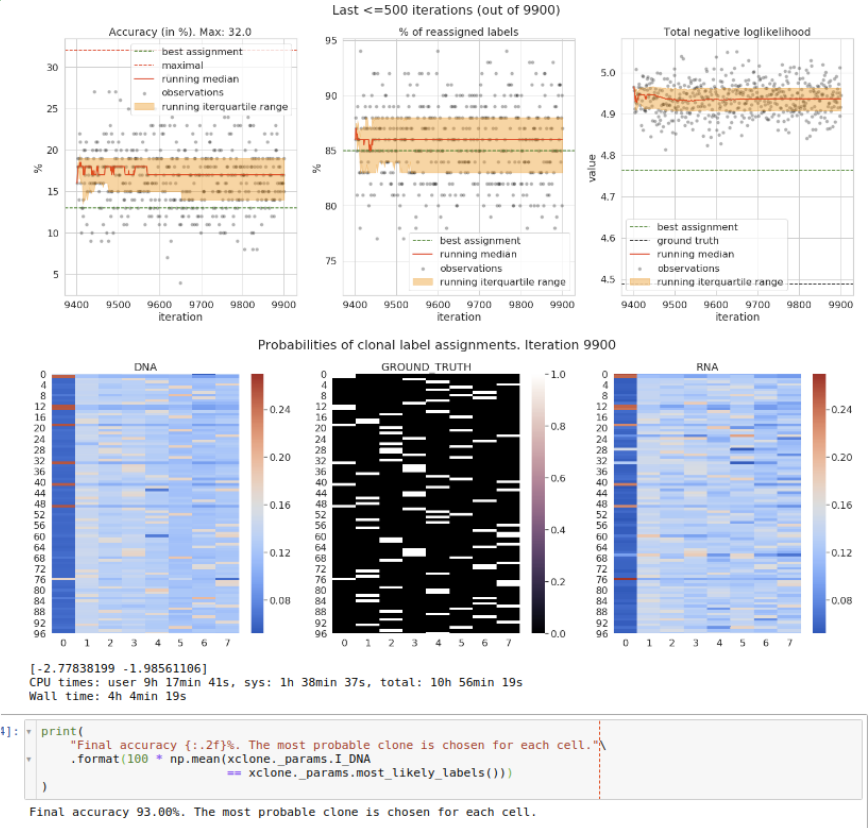
\includegraphics[keepaspectratio=true, scale=0.5]{images/xclone_v1_simulated_data_convergence_monitor.png}
	\caption{Рукописная визуализация процесса обучения XClone-V1, последние 500 итераций. Строкам тепловых карт в нижнем ряду соответствуют клетки, столбцам — клональные линии, а ячейке на позиции $(j, k)$ — вероятность того, что клетка $j$ принадлежит линии $k$. Центральная карта показывает истинные клональные линии, левая — вероятности, подсчитанные по scDNA-seq, правая — по scRNA-seq. Верхние тепловые карты позволяют, как распределения из нижних тепловых карт менялись в ходе обучения. Левая карта показывает точность предсказания, если клональная линии назначается случайно в соответствии с текущим распределением вероятностей на метках. Центральная карта показывает, какой процент меток при таком подходе отличается от расстановки, полученной 100 итераций назад. Правая карта показывает, как менялся минус логарифм функции правдподобия от итерации к итерации.}
\end{figure}

\begin{figure}[H]
	\centering
	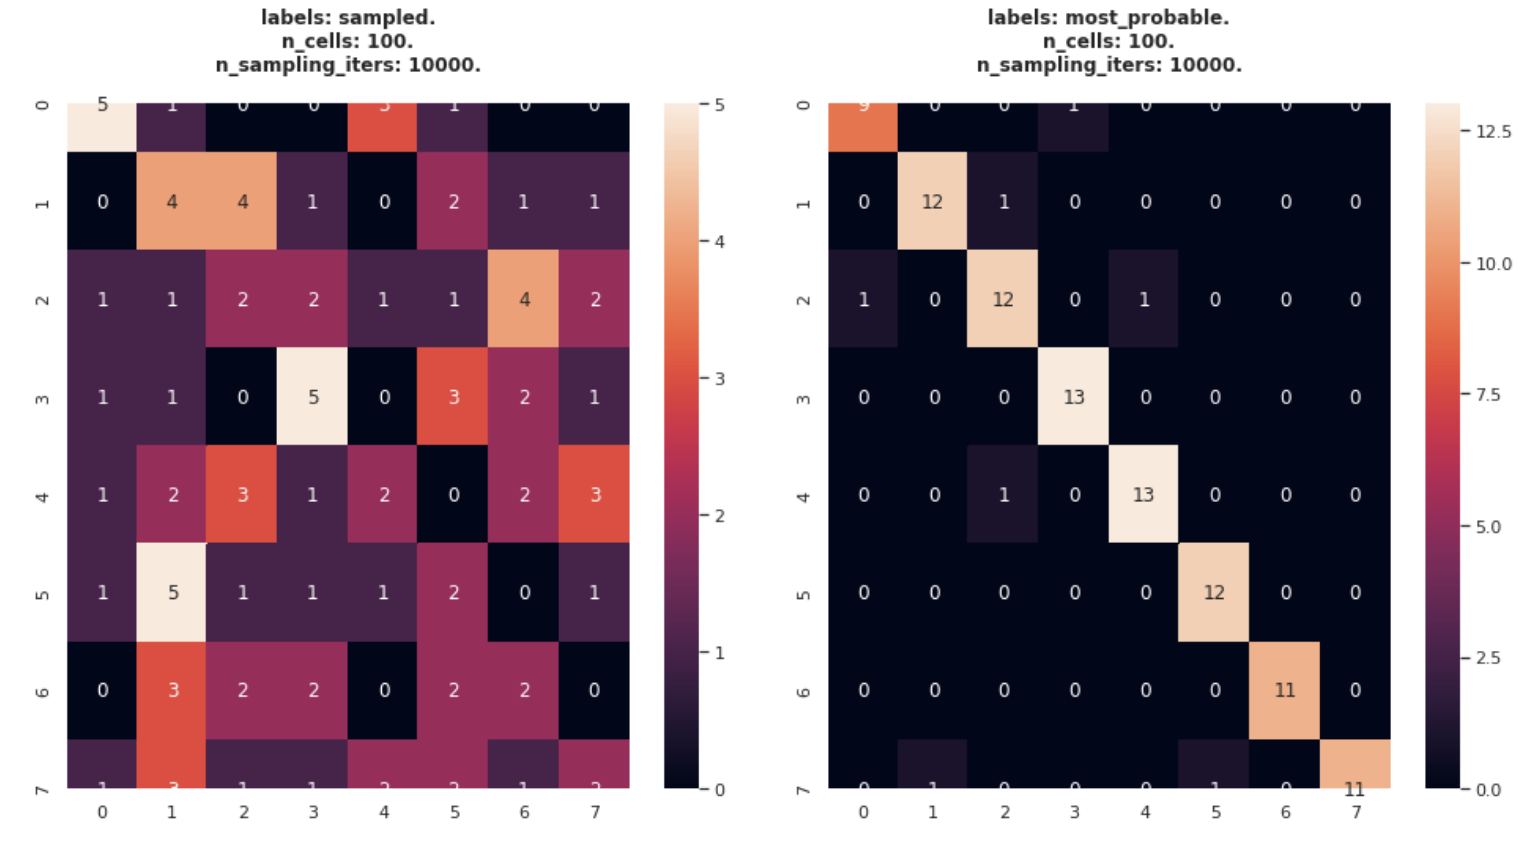
\includegraphics[keepaspectratio=true, scale=0.3]{images/xclone_v1_simulated_data_confusion_matrices.png}
	\caption{Матрицы ошибок (confusion matrix) для предсказанных клональных линий. Слева — метки, полученные семплированием, справа — моды соответствующих распределений.}
\end{figure}
По графикам видно, что алгоритм находит правильные метки, но не очень уверен в них. С ростом глубины покрытия при генерции клеток эта проблема становилась менее выраженной, но и синтетические данные при этом всё меньше напоминали реальные. Симуляция показала, что для надёжной работы алгоритма нужны были РНК-данные гораздо более высокого качества, чем в образцах от DKFZ. Кроме того, итоговая точность сильно зависела от качества BAF-сигнала, который в РНК-образцах раз за разом оказывался слишком зашумленным. Именно в связи с этим и была разработана XClone-V2, где во главе угла не BAF, а RDR.

Эксперименты для валидации XClone-V2 устроен аналогично, разве что добавляется информация о числе всех прочтений $\bm{R_{j}}$. Кроме того, теперь нужно генерировать ASCNV. Доля затронутых ими блоков сегментации в каждом из клонов задаётся пользователем, равно как и частоты отдельных аллель-специфических конфигураций $(c_{t,m}, c_{t,p})$. 
\begin{figure}[H]
	\centering
	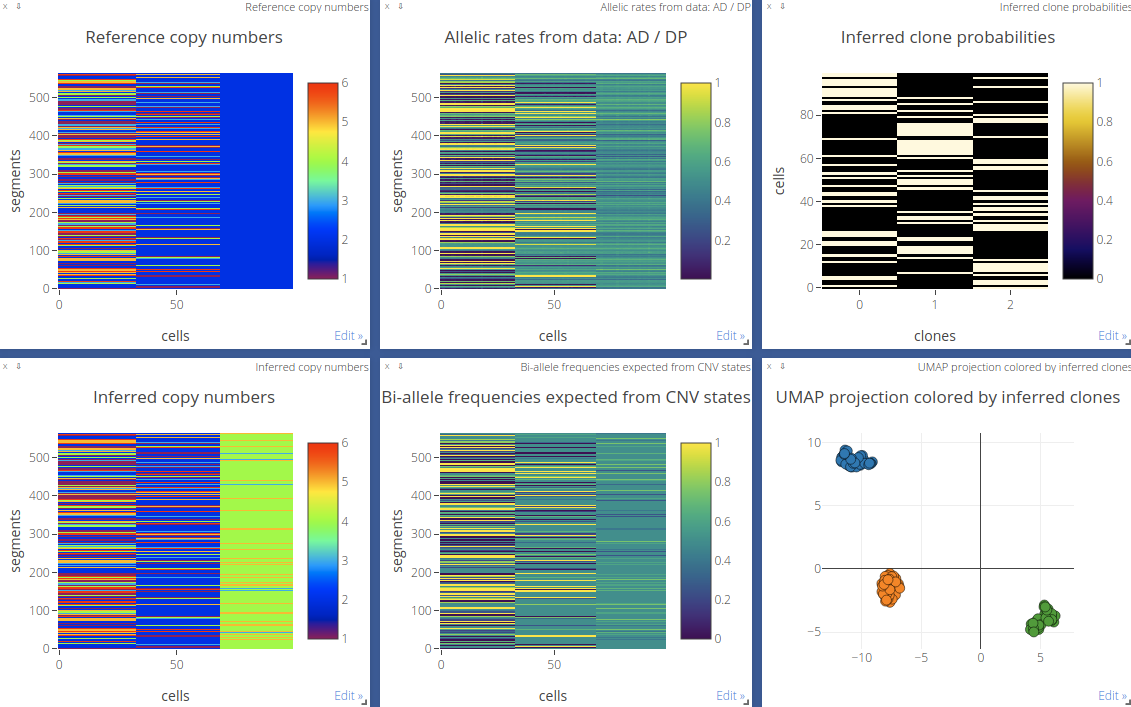
\includegraphics[keepaspectratio=true, scale=0.4]{images/xclone_v2_simulation_results.png}
	\caption{Визуализация процесса обучения XClone-V2, выполненная в Visdom от Facebook Research. Тепловые карты в верхней строке, слева направо: истинные клональные RDR- и BAF-сигналы, а также вероятности принадлежности клеток клональным линиям (все сошлись к истинным). Нижняя строка, слева направо: предсказанное число копий в каждом из клонов, предсказанный аллельный дисбаланс и проекция клеток конкатенации этих двух векторов на 2D с помощью алгоритма UMAP, где каждый цвет соответствует клональной линии.}
\end{figure}
Скачок качества очевиден: корректное распределение на метках клональных линий удаётся получить всего за пару десятков итераций VB, чего в XClone-V1 не удавалось достичь даже за 10000 итераций семплирования по Гиббсу.

При этом бросается в глаза, что модель сильно ошибается на нормальных клетках: она предсказывает WGD там, где его нет. Но ранее упоминалось, что мультиномиальная модель RDR-модуля в XClone-V2 не позволяет детектировать WGD, потому на стадии байесовского вывода такие ошибки неизбежны. Их можно попытаться скорректировать на стадии пост-обработки, об этом можно прочесть в заключительном разделе ВКР. В остальном же и BAF-, и RDR-модуль предсказывают корректные величины.

Кроме того, справедливо будет заметить, что пока что эксперименты не позволяют оценить качество модели как классификатора. В идеальных условиях незашумленных BAF- и RDR-сигналов в данных классифицировать клетки просто: видно, что клональные линии линейно разделимы при проекции на 2D. Алгоритм KMeans в таком случае тоже даёт 100\% точность. Поэтому симуляции сейчас проверяют не то, как классифицируются клетки, а как модель восстанавливает ASCNV. Сейчас это не первоочередная задача, но в последующих версиях модели будут реализованы и более продвинутые подходы к генерации данных. 

\subsection{Реальные данные: STP, scDNA-seq}
\begin{figure}[H]
	\centering
	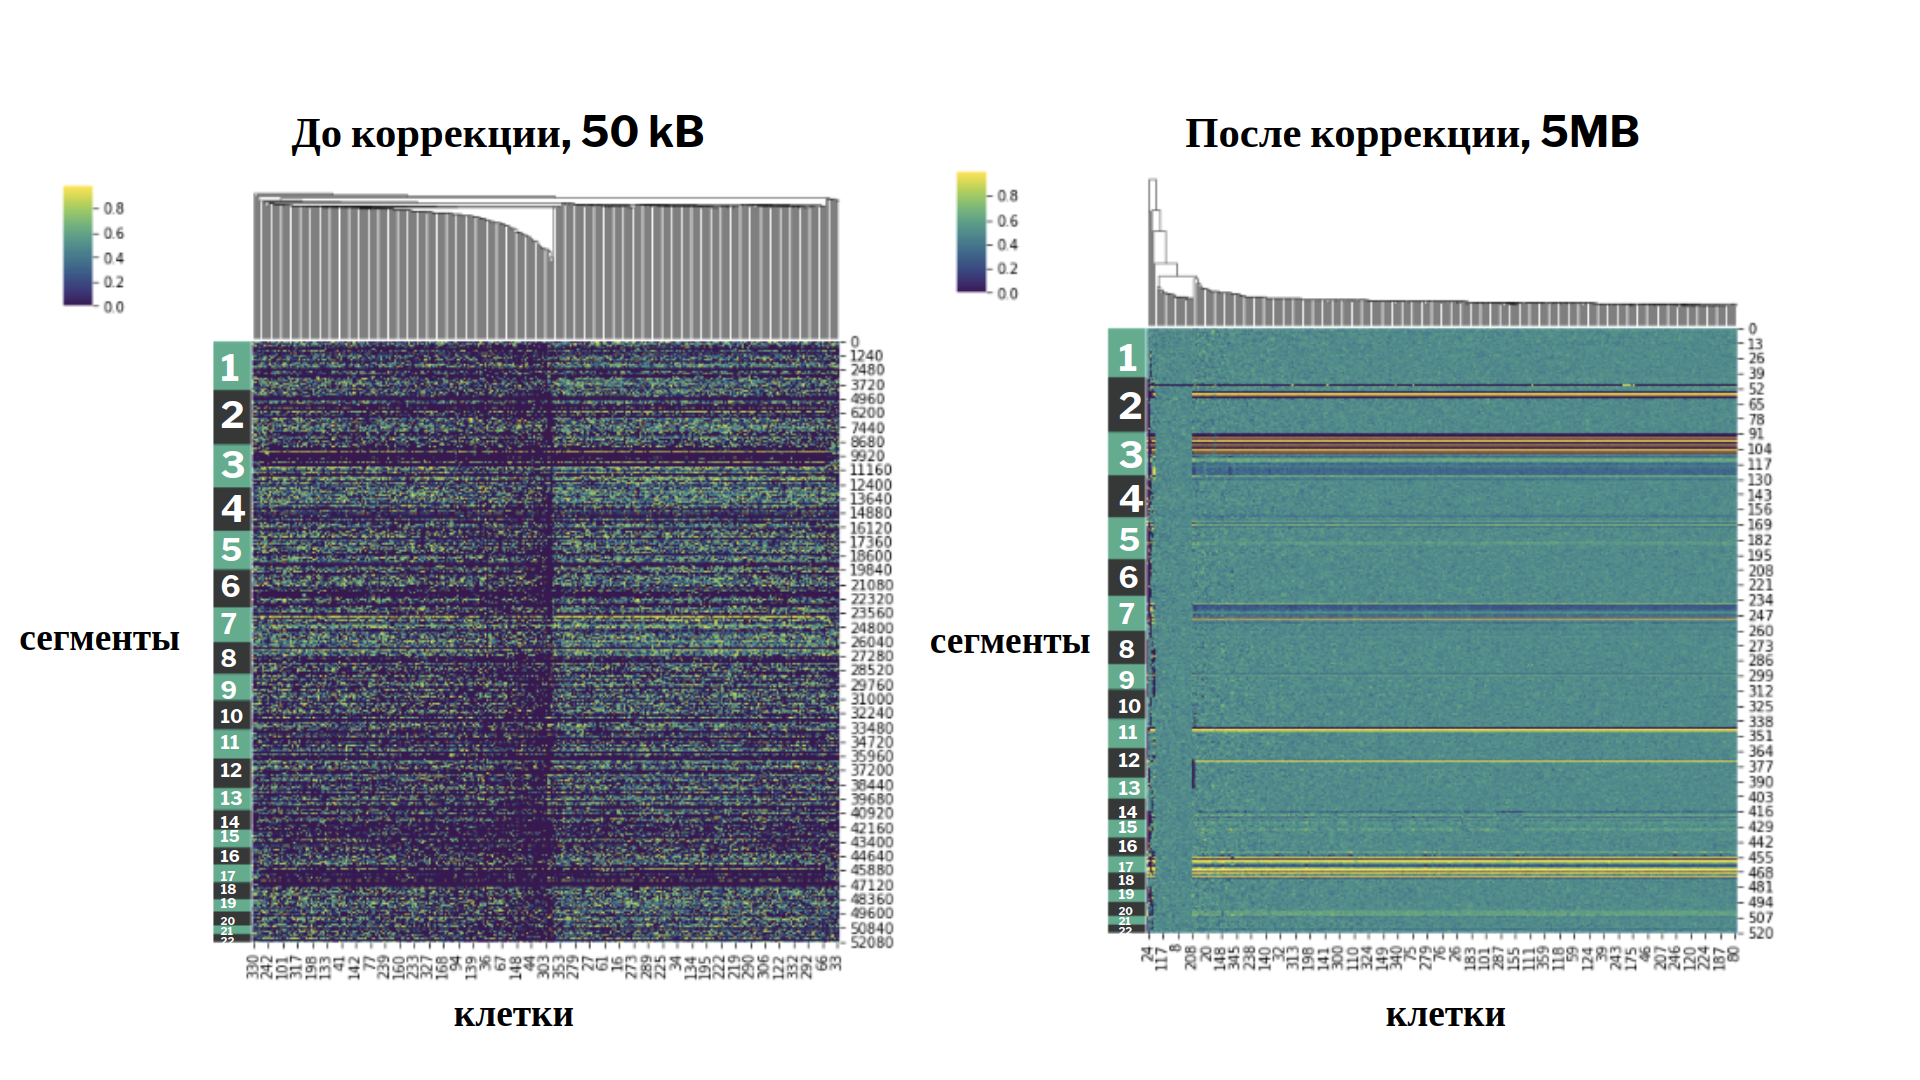
\includegraphics[keepaspectratio=true,scale=0.2]{images/bin_linkage_stp_nuclei_dna.png}
	\caption{Коррекция ошибок смены цепи на примере ДНК-образца медуллобластомы, STP-Nuclei. На рисунке изображены тепловые карты долей аллеля из <<материнского>> гаплотипа, числа слева обозначают номер хромосомы. Картина аллельного дисбаланса до коррекции практически не прослеживается, после — становится очевидна.}
\end{figure}

\begin{figure}[H]
	\centering
	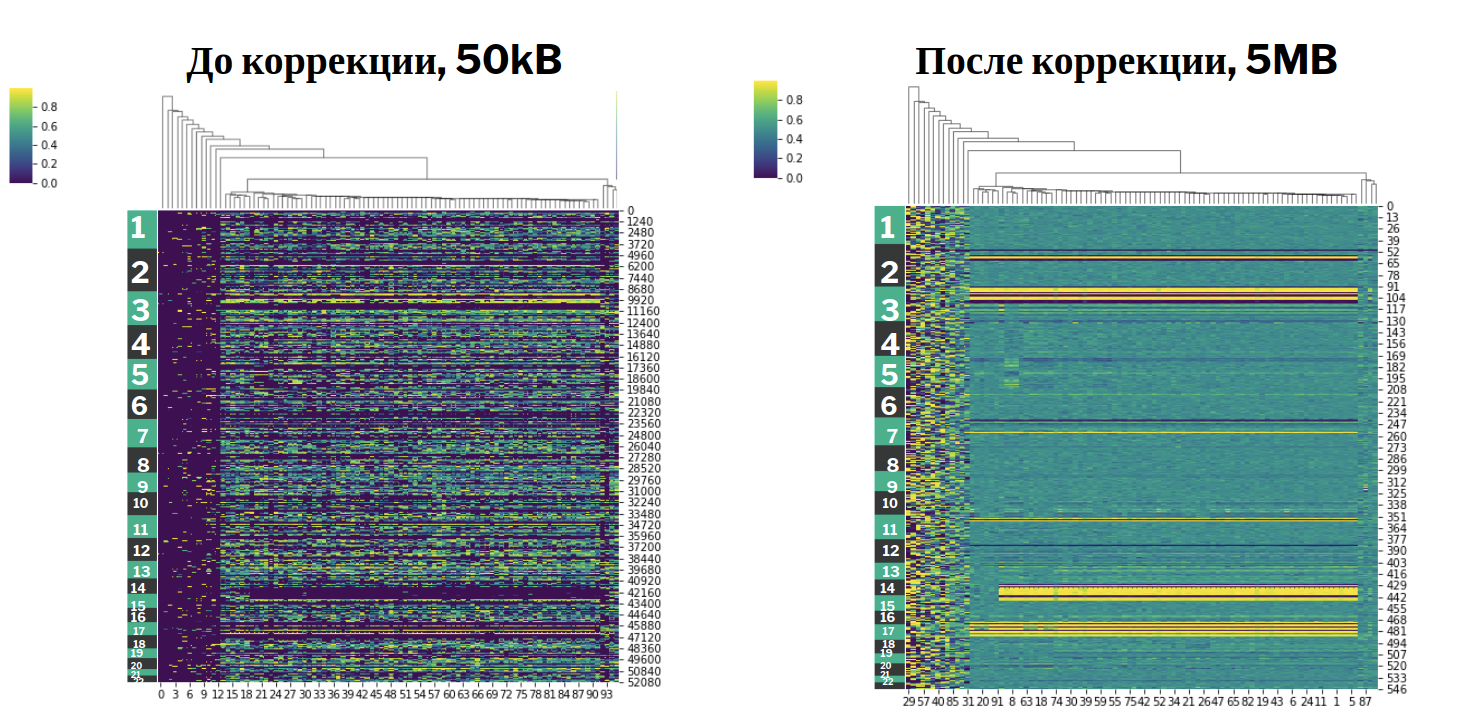
\includegraphics[keepaspectratio=true,scale=0.2]{images/bin_linkage_stp_gt_dna.png}
	\caption{Коррекция ошибок смены цепи на примере ДНК-образца медуллобластомы, STP-G\&T. Суть та же, что и на предыдущей иллюстрации, но в этом образце глубина покрытия клеток в среднем выше, а потому аллельный сигнал проступает и в масштабе 50 килобаз.}
\end{figure}

\subsection{Реальные данные: STP, scRNA-seq}
Как уже упоминалось ранее, изначально XClone задумывался как метод совместного анализа нескольких омик. В планах было увязать друг с другом хотя бы геномные и транскриптомные данные: определять клональную структуру опухоли по scDNA-seq, а потом классифицировать по клональным линиям клетки последовательных scRNA-seq образцов и следить за эволюцией опухоли в динамике. Это позволило бы лучше понимать, как опухоль реагирует на лечение. Если бы метод работал надёжно, то он мог бы стать ценным инструментом в руках врачей-онкологов.

Но интеграция нескольких single-cell омик неспроста считается одной из 11 главных задач анализа single-cell данных \cite{ElevenGrandChallengesInSingleCellDS}. Первые результаты выглядели вдохновляюще:

\begin{figure}[H]
	\centering
	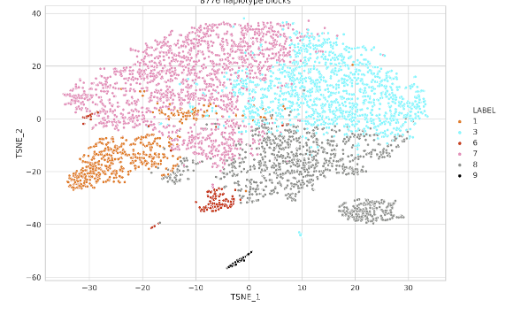
\includegraphics[keepaspectratio=true,scale=0.8]{images/xclone_v1_stp_nuclei_rna_clones_tsne.png}
	\caption{Клетки РНК-образца, STP-Nuclei. Цвет соответствует клональной линии, предсказанной XClone-V1. Большой кластер точек по центру — опухолевые клетки, кластер снизу справа — нормальные клетки, природу малых кластеров в нижней части рисунка установить не удалось.}
\end{figure}

\begin{figure}[H]
	\centering
	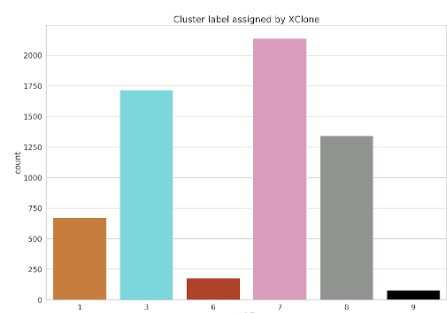
\includegraphics[keepaspectratio=true,scale=0.8]{images/xclone_v1_stp_nuclei_rna_clones_hist.png}
	\caption{Клетки РНК-образца, STP-Nuclei. Гистограммы предсказанных классов на предыдущем рисунке.}
\end{figure}

Да, часть опухолевых клеток была размечена как нормальные, но изначально это списали на то, что в данных могла быть примесь других клеточных типов, которые по профилю транскрипции находятся где-то между нормальными и опухолевыми. Тем не менее, систематический перебор random seed показал, что пропорции предсказанных классов, равно как и их количество и размеры, меняются в слишком больших пределах. Проще говоря, траскриптомных данных было слишком мало, чтобы получить достаточно хороший BAF-сигнал. 

Предпринималось много попыток сгруппировать гетерозиготные ОНП так, чтобы суммарный сигнал был достаточно сильным для уверенной классификации. Тем не менее, все они упирались в проблемы статистического фазирования гаплотипов, причём как статистического, так и основанного на длинных прочтениях, полученных по технологии Oxford Nanopore. Тем не менее, работа продолжалась. Большие надежды возлагались на разработанный метод коррекции ошибок смены цепи, который зарекомендовал себя на данных scDNA-seq образцов STP-Nuclei и STP-G\&T.

Тем не менее, scRNA-seq данные STP-Nuclei оставались слишком разреженными даже в масштабе десятков мегабаз, когда предсказание числа копий уже теряло содержательный смысл:

\begin{figure}[H]
	\centering
	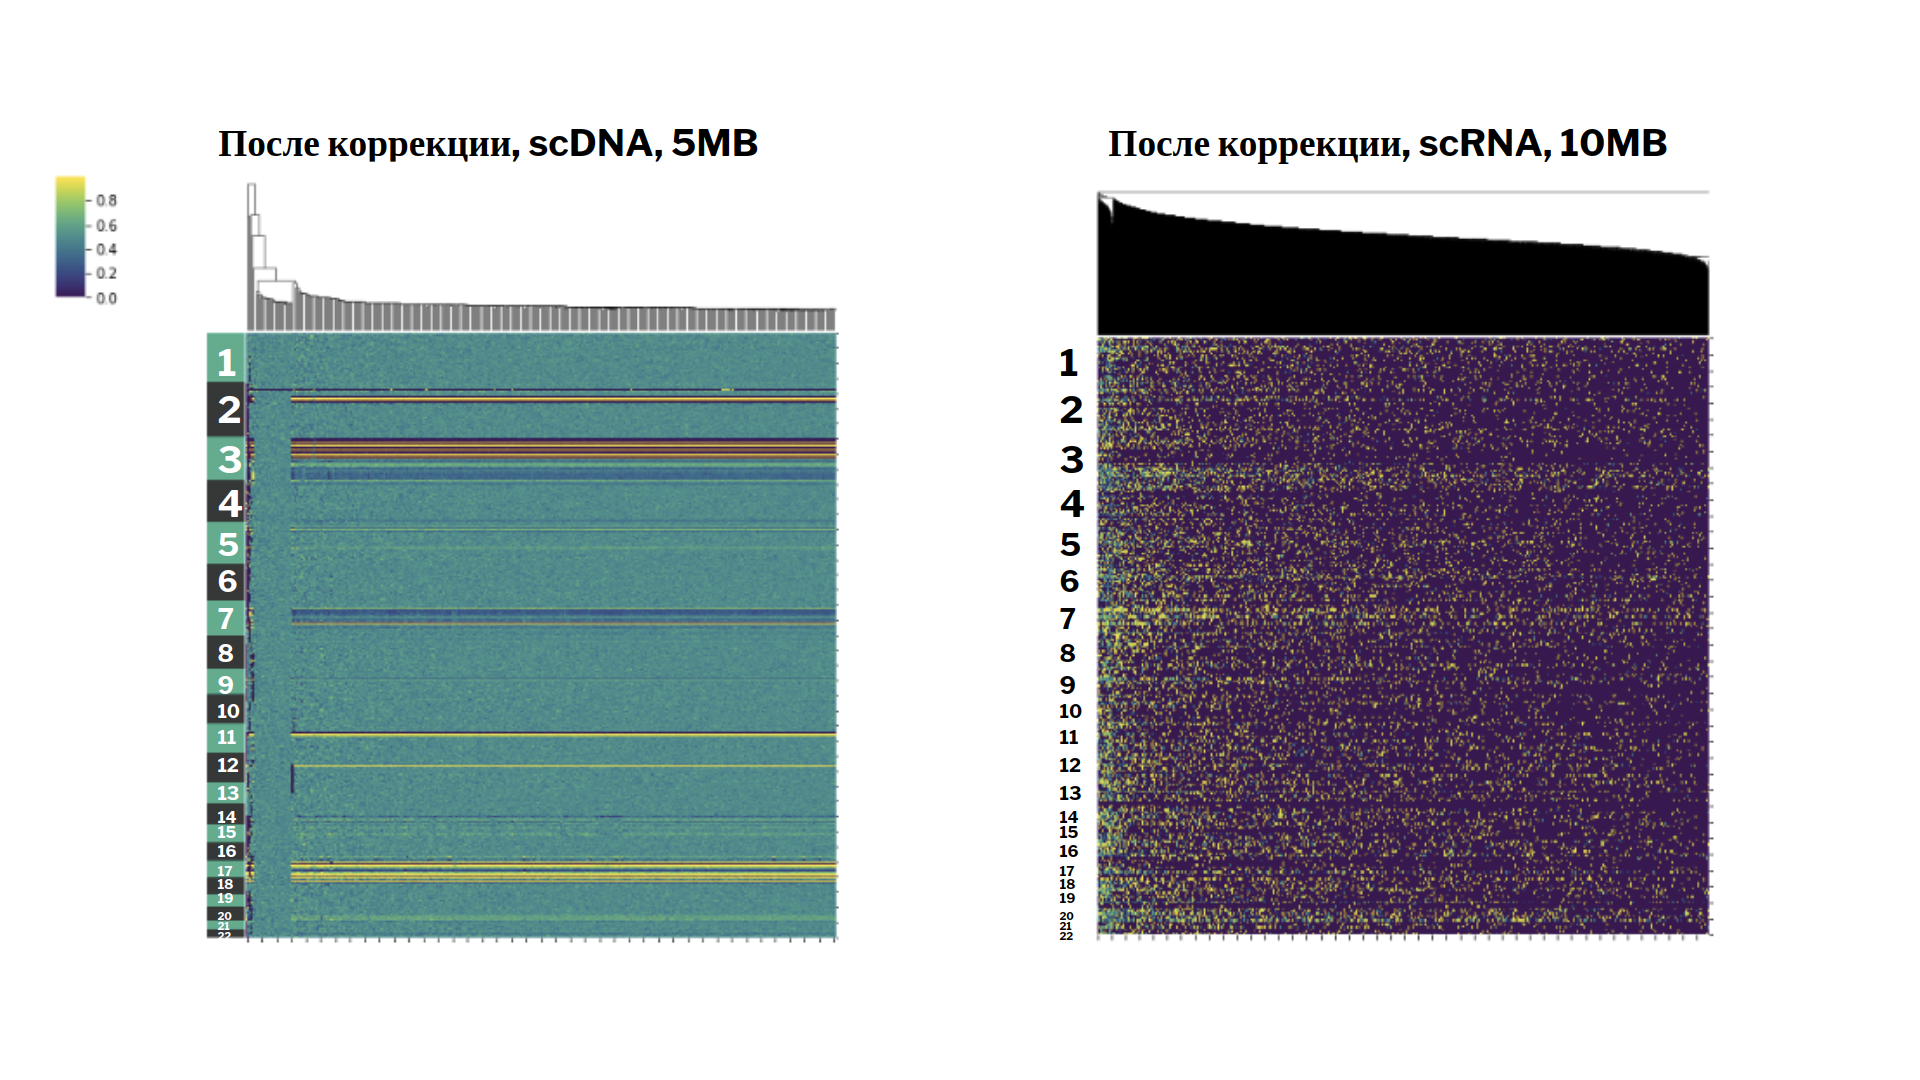
\includegraphics[keepaspectratio=true,scale=0.25]{images/bin_linkage_stp_nuclei_dna_rna.png}
	\caption{Попытка коррекция ошибок смены цепи на примере ДНК- и РНК-образцов медуллобластомы, STP-Nuclei. Здесь фиолетовый цвет означает "нет данных". Даже в масштабе 10 мегабаз структура аллельного дисбаланса в данных РНК-секвенирования практически не просматривается.}
\end{figure}

Несмотря на то, что РНК-данные из STP-G\&T гораздо менее разреженные, чем РНК-данные из STP-Nuclei, структура аллельного дисбаланса в них тоже не просматривалась:

\begin{figure}[H]
	\centering
	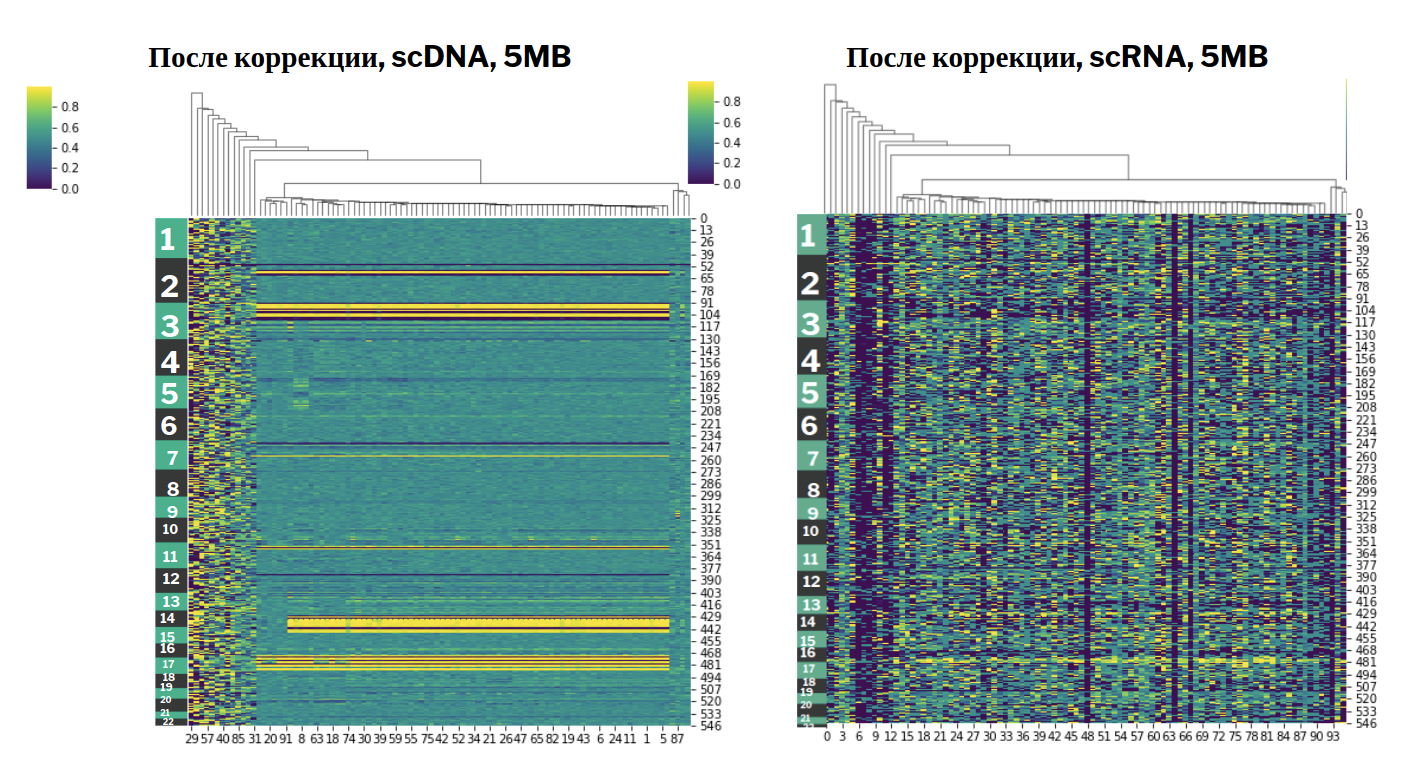
\includegraphics[keepaspectratio=true,scale=0.25]{images/bin_linkage_stp_gt_dna_rna.png}
	\caption{Попытка коррекция ошибок смены цепи на примере ДНК- и РНК-образцов медуллобластомы, STP-G\&T. Порядок клеток одинаков на обеих тепловых картах.}
\end{figure}

